\documentclass[12pt,twoside]{article}

\newcommand{\reporttitle}{Deep Learning For Facial Expression Analysis}
\newcommand{\reportauthor}{Tom Bartissol}
\newcommand{\reporttype}{Interim Report}
\newcommand{\cid}{00824562}

% paragraph skip length
\setlength{\parskip}{1em}
% line spacing
\renewcommand{\baselinestretch}{1.1}
\newcommand{\source}[1]{\vspace{-3pt} \caption*{ \footnotesize{\textit{Source: {#1}}}} }


% include files that load packages and define macros
%%%%%%%%%%%%%%%%%%%%%%%%%%%%%%%%%%%%%%%%%
% University Assignment Title Page 
% LaTeX Template
% Version 1.0 (27/12/12)
%
% This template has been downloaded from:
% http://www.LaTeXTemplates.com
%
% Original author:
% WikiBooks (http://en.wikibooks.org/wiki/LaTeX/Title_Creation)
%
% License:
% CC BY-NC-SA 3.0 (http://creativecommons.org/licenses/by-nc-sa/3.0/)
% 
% Instructions for using this template:
% This title page is capable of being compiled as is. This is not useful for 
% including it in another document. To do this, you have two options: 
%
% 1) Copy/paste everything between \begin{document} and \end{document} 
% starting at \begin{titlepage} and paste this into another LaTeX file where you 
% want your title page.
% OR
% 2) Remove everything outside the \begin{titlepage} and \end{titlepage} and 
% move this file to the same directory as the LaTeX file you wish to add it to. 
% Then add \input{./title_page_1.tex} to your LaTeX file where you want your
% title page.
%
%----------------------------------------------------------------------------------------
%	PACKAGES AND OTHER DOCUMENT CONFIGURATIONS
%----------------------------------------------------------------------------------------
\usepackage{ifxetex}
\usepackage{textpos}
\usepackage{natbib}
\usepackage{kpfonts}
\usepackage[a4paper,hmargin=2.8cm,vmargin=2.0cm,includeheadfoot]{geometry}
\usepackage{ifxetex}
\usepackage{stackengine}
\usepackage{tabularx,longtable,multirow,caption}%hangcaption
\usepackage{fncylab} %formatting of labels
\usepackage{fancyhdr}
\usepackage{color}
\usepackage[tight,ugly]{units}
\usepackage{url}
\usepackage{float}
\usepackage[english]{babel}
\usepackage{amsmath}
\usepackage{graphicx}
\usepackage[colorinlistoftodos]{todonotes}
\usepackage{dsfont}
\usepackage{epstopdf} % automatically replace .eps with .pdf in graphics
\usepackage{natbib}
\usepackage{backref}
\usepackage{array}
\usepackage{latexsym}
\usepackage{etoolbox}

\usepackage{enumerate} % for numbering with [a)] format 



\ifxetex
\usepackage{fontspec}
\setmainfont[Scale=.8]{OpenDyslexic-Regular}
\else
\usepackage[pagebackref,hypertexnames=false,colorlinks]{hyperref} % provide links in pdf
\hypersetup{pdftitle={},
  pdfsubject={}, 
  pdfauthor={\reportauthor},
  pdfkeywords={}, 
  pdfstartview=FitH,
  pdfpagemode={UseOutlines},% None, FullScreen, UseOutlines
  bookmarksnumbered=true, bookmarksopen=true, colorlinks,
    citecolor=green,%
    filecolor=black,%
    linkcolor=black,%
    urlcolor=black}
\usepackage[all]{hypcap}
\fi

\usepackage{tcolorbox}

% various theorems
\usepackage{ntheorem}
\theoremstyle{break}
\newtheorem{lemma}{Lemma}
\newtheorem{theorem}{Theorem}
\newtheorem{remark}{Remark}
\newtheorem{definition}{Definition}
\newtheorem{proof}{Proof}

% example-environment
\newenvironment{example}[1][]
{ 
\vspace{4mm}
\noindent\makebox[\linewidth]{\rule{\hsize}{1.5pt}}
\textbf{Example #1}\\
}
{ 
\noindent\newline\makebox[\linewidth]{\rule{\hsize}{1.0pt}}
}



%\renewcommand{\rmdefault}{pplx} % Palatino
% \renewcommand{\rmdefault}{put} % Utopia

\ifxetex
\else
\renewcommand*{\rmdefault}{bch} % Charter
\renewcommand*{\ttdefault}{cmtt} % Computer Modern Typewriter
%\renewcommand*{\rmdefault}{phv} % Helvetica
%\renewcommand*{\rmdefault}{iwona} % Avant Garde
\fi

\setlength{\parindent}{4em}  % indentation of paragraph

\setlength{\headheight}{14.5pt}
\pagestyle{fancy}
\fancyfoot[ER,OL]{\thepage}%Page no. in the left on
                                %odd pages and on right on even pages
\fancyfoot[OC,EC]{\sffamily }
\renewcommand{\headrulewidth}{0.1pt}
\renewcommand{\footrulewidth}{0.1pt}
\captionsetup{margin=10pt,font=small,labelfont=bf}


%--- chapter heading

\def\@makechapterhead#1{%
  \vspace*{10\p@}%
  {\parindent \z@ \raggedright %\sffamily
        %{\Large \MakeUppercase{\@chapapp} \space \thechapter}
        %\\
        %\hrulefill
        %\par\nobreak
        %\vskip 10\p@
    \interlinepenalty\@M
    \Huge \bfseries 
    \thechapter \space\space #1\par\nobreak
    \vskip 30\p@
  }}

%---chapter heading for \chapter*  
\def\@makeschapterhead#1{%
  \vspace*{10\p@}%
  {\parindent \z@ \raggedright
    \sffamily
    \interlinepenalty\@M
    \Huge \bfseries  
    #1\par\nobreak
    \vskip 30\p@
  }}
  



% %%%%%%%%%%%%% boxit
\def\Beginboxit
   {\par
    \vbox\bgroup
	   \hrule
	   \hbox\bgroup
		  \vrule \kern1.2pt %
		  \vbox\bgroup\kern1.2pt
   }

\def\Endboxit{%
			      \kern1.2pt
		       \egroup
		  \kern1.2pt\vrule
		\egroup
	   \hrule
	 \egroup
   }	

\newenvironment{boxit}{\Beginboxit}{\Endboxit}
\newenvironment{boxit*}{\Beginboxit\hbox to\hsize{}}{\Endboxit}



\allowdisplaybreaks

\makeatletter
\newcounter{elimination@steps}
\newcolumntype{R}[1]{>{\raggedleft\arraybackslash$}p{#1}<{$}}
\def\elimination@num@rights{}
\def\elimination@num@variables{}
\def\elimination@col@width{}
\newenvironment{elimination}[4][0]
{
    \setcounter{elimination@steps}{0}
    \def\elimination@num@rights{#1}
    \def\elimination@num@variables{#2}
    \def\elimination@col@width{#3}
    \renewcommand{\arraystretch}{#4}
    \start@align\@ne\st@rredtrue\m@ne
}
{
    \endalign
    \ignorespacesafterend
}
\newcommand{\eliminationstep}[2]
{
    \ifnum\value{elimination@steps}>0\leadsto\quad\fi
    \left[
        \ifnum\elimination@num@rights>0
            \begin{array}
            {@{}*{\elimination@num@variables}{R{\elimination@col@width}}
            |@{}*{\elimination@num@rights}{R{\elimination@col@width}}}
        \else
            \begin{array}
            {@{}*{\elimination@num@variables}{R{\elimination@col@width}}}
        \fi
            #1
        \end{array}
    \right]
    & 
    \begin{array}{l}
        #2
    \end{array}
    &%                                    moved second & here
    \addtocounter{elimination@steps}{1}
}
\makeatother

%% Fast macro for column vectors
\makeatletter  
\def\colvec#1{\expandafter\colvec@i#1,,,,,,,,,\@nil}
\def\colvec@i#1,#2,#3,#4,#5,#6,#7,#8,#9\@nil{% 
  \ifx$#2$ \begin{bmatrix}#1\end{bmatrix} \else
    \ifx$#3$ \begin{bmatrix}#1\\#2\end{bmatrix} \else
      \ifx$#4$ \begin{bmatrix}#1\\#2\\#3\end{bmatrix}\else
        \ifx$#5$ \begin{bmatrix}#1\\#2\\#3\\#4\end{bmatrix}\else
          \ifx$#6$ \begin{bmatrix}#1\\#2\\#3\\#4\\#5\end{bmatrix}\else
            \ifx$#7$ \begin{bmatrix}#1\\#2\\#3\\#4\\#5\\#6\end{bmatrix}\else
              \ifx$#8$ \begin{bmatrix}#1\\#2\\#3\\#4\\#5\\#6\\#7\end{bmatrix}\else
                 \PackageError{Column Vector}{The vector you tried to write is too big, use bmatrix instead}{Try using the bmatrix environment}
              \fi
            \fi
          \fi
        \fi
      \fi
    \fi
  \fi 
}  
\makeatother

\robustify{\colvec}

%%% Local Variables: 
%%% mode: latex
%%% TeX-master: "notes"
%%% End: 
 % various packages needed for maths etc.
% quick way of adding a figure
\newcommand{\fig}[3]{
 \begin{center}
 \scalebox{#3}{\includegraphics[#2]{#1}}
 \end{center}
}

%\newcommand*{\point}[1]{\vec{\mkern0mu#1}}
\newcommand{\ci}[0]{\perp\!\!\!\!\!\perp} % conditional independence
\newcommand{\point}[1]{{#1}} % points 
\renewcommand{\vec}[1]{{\boldsymbol{{#1}}}} % vector
\newcommand{\mat}[1]{{\boldsymbol{{#1}}}} % matrix
\newcommand{\R}[0]{\mathds{R}} % real numbers
\newcommand{\Z}[0]{\mathds{Z}} % integers
\newcommand{\N}[0]{\mathds{N}} % natural numbers
\newcommand{\nat}[0]{\mathds{N}} % natural numbers
\newcommand{\Q}[0]{\mathds{Q}} % rational numbers
\ifxetex
\newcommand{\C}[0]{\mathds{C}} % complex numbers
\else
\newcommand{\C}[0]{\mathds{C}} % complex numbers
\fi
\newcommand{\tr}[0]{\text{tr}} % trace
\renewcommand{\d}[0]{\mathrm{d}} % total derivative
\newcommand{\inv}{^{-1}} % inverse
\newcommand{\id}{\mathrm{id}} % identity mapping
\renewcommand{\dim}{\mathrm{dim}} % dimension
\newcommand{\rank}[0]{\mathrm{rk}} % rank
\newcommand{\determ}[1]{\mathrm{det}(#1)} % determinant
\newcommand{\scp}[2]{\langle #1 , #2 \rangle}
\newcommand{\kernel}[0]{\mathrm{ker}} % kernel/nullspace
\newcommand{\img}[0]{\mathrm{Im}} % image
\newcommand{\idx}[1]{{(#1)}}
\DeclareMathOperator*{\diag}{diag}
\newcommand{\E}{\mathds{E}} % expectation
\newcommand{\var}{\mathds{V}} % variance
\newcommand{\gauss}[2]{\mathcal{N}\big(#1,\,#2\big)} % gaussian distribution N(.,.)
\newcommand{\gaussx}[3]{\mathcal{N}\big(#1\,|\,#2,\,#3\big)} % gaussian distribution N(.|.,.)
\newcommand{\gaussBig}[2]{\mathcal{N}\left(#1,\,#2\right)} % see above, but with brackets that adjust to the height of the arguments
\newcommand{\gaussxBig}[3]{\mathcal{N}\left(#1\,|\,#2,\,#3\right)} % see above, but with brackets that adjust to the height of the arguments
\DeclareMathOperator{\cov}{Cov} % covariance (matrix) 
\ifxetex
\renewcommand{\T}[0]{^\top} % transpose
\else
\newcommand{\T}[0]{^\top}
\fi
% matrix determinant
\newcommand{\matdet}[1]{
\left|
\begin{matrix}
#1
\end{matrix}
\right|
}



%%% various color definitions
\definecolor{darkgreen}{rgb}{0,0.6,0}

\newcommand{\blue}[1]{{\color{blue}#1}}
\newcommand{\red}[1]{{\color{red}#1}}
\newcommand{\green}[1]{{\color{darkgreen}#1}}
\newcommand{\orange}[1]{{\color{orange}#1}}
\newcommand{\magenta}[1]{{\color{magenta}#1}}
\newcommand{\cyan}[1]{{\color{cyan}#1}}


% redefine emph
\renewcommand{\emph}[1]{\blue{\bf{#1}}}

% place a colored box around a character
\gdef\colchar#1#2{%
  \tikz[baseline]{%
  \node[anchor=base,inner sep=2pt,outer sep=0pt,fill = #2!20] {#1};
    }%
}%
 % short-hand notation and macros


\usepackage[toc,page]{appendix}

%%%%%%%%%%%%%%%%%%%%%%%%%%%%

\begin{document}
% front page
% Last modification: 2016-09-29 (Marc Deisenroth)
\begin{titlepage}

\newcommand{\HRule}{\rule{\linewidth}{0.5mm}} % Defines a new command for the horizontal lines, change thickness here


%----------------------------------------------------------------------------------------
%	LOGO SECTION
%----------------------------------------------------------------------------------------


\includegraphics[width = 4cm]{./figures/imperial.eps}\\[0.5cm] 

\begin{center} % Center remainder of the page

%----------------------------------------------------------------------------------------
%	HEADING SECTIONS
%----------------------------------------------------------------------------------------
\textsc{\LARGE \reporttype}\\[1.5cm] 
\textsc{\Large Imperial College London}\\[0.5cm] 
\textsc{\large Department of Computing}\\[0.5cm] 
%----------------------------------------------------------------------------------------
%	TITLE SECTION
%----------------------------------------------------------------------------------------

\HRule \\[0.4cm]
{ \huge \bfseries \reporttitle}\\ % Title of your document
\HRule \\[1.5cm]
\end{center}
%----------------------------------------------------------------------------------------
%	AUTHOR SECTION
%----------------------------------------------------------------------------------------

%\begin{minipage}{0.4\hsize}
\begin{flushleft} \large
\textit{Author:}\\
\reportauthor~(CID: \cid) % Your name
\end{flushleft}
\vspace{2cm}
\makeatletter
Date: \@date 

\vfill % Fill the rest of the page with whitespace



\makeatother


\end{titlepage}



\tableofcontents
\clearpage
%%%%%%%%%%%%%%%%%%%%%%%%%%%% Main document

\section{Introduction}

The ability to analyse human facial expressions is an active area of research with exciting near-future real-world applications ranging from law enforcement to advertising (measuring how positively or negatively people respond to an ad). It would also be at the core of any system capable of intelligent Human-Computer Interaction (HCI). Indeed, for such interactions to be life-like, the Computer should be able to recognise human emotions which are expressed through multiple channels, an important one being facial expressions. \textit{Interpreting} the recognised facial expressions into the six \textit{basic emotions} \cite{RefWorks:12} (see Table ~\ref{tab:emo-au}) would allow the Computer to identify human emotions to some extent.

Facial Expressions result from the contraction of a facial muscle or a group of facial muscles and the visually perceptible changes due to such contractions have been codified by Ekman and Friesen into the well-known Facial Action Coding System (FACS) \cite{RefWorks:10} which provides labels, facial \textit{Action Units} (AUs), for the actions of a muscle or group of muscles. For instance, AU 12 corresponds the lip corner puller and if it is active at the same time as AU 6, which corresponds to the cheek raiser, then the subject is smiling and this could be interpreted as happiness.

We are therefore concerned with two problems (i) identifying these AUs and (ii) estimating continuous emotion dimensions: valence (how positive or negative the emotion is) and arousal (how intense) instead of discrete emotions such as the six basic emotions. Since changes in muscular activity are not instant but last between 250ms and 5s \cite{RefWorks:11}, we are interested in data with a temporal dimension, that is videos. More specifically, whereas the majority of previous work has been conducted on data sets captured in constrained environment and/or using acted or posed facial expressions \cite{RefWorks:2}, we are interested in the so called "\textit{in-the-wild}" videos, which are recorded in different lighting conditions with different poses and most accurately represent spontaneous facial expressions.

To achieve this, we will use end-to-end deep learning models, namely ResNet, VGG and ResNet-Inception. Each model will be trained/fine tuned to jointly solve problems (i) and (ii) on data taken in-the-wild. Finally we will evaluate these models on existing and established benchmarks and databases (not necessarily in-the-wild).


\clearpage
\section{Background}

\subsection{Facial Expressions}

\subsubsection{Facial Action Coding System (FACS)}

The human head having a finite number of muscles, the number of visually perceptible changes that can be caused by the contraction or relaxation of one or more of these muscles, that is the number of facial expressions, is finite. We can therefore taxonomise these facial changes into a coding system. Although there exists a few such coding systems \cite{RefWorks:13}, the most popular and used coding system is the FACS \cite{RefWorks:10}. FACS breaks down each visually perceptible change into facial \textit{Action Units} (AUs) which roughly corresponds to the contraction or relaxation of individual facial muscles. The activation of one or more AU creates a facial expression. Some examples of AUs and their associated facial are listed in Figure ~\ref{fig:fau}.

On top of this taxonomy, FACS also provides an intensity score, A-E (maximum-minimum), to rate how pronounced each AU is in a facial expression (see Table ~\ref{tab:scale-au}). For instance AU 12A would indicate that the lip corners are slightly pulled whereas AU 12E would indicate that they are maximally pulled.

Finally, AUs do not activate instantly. Indeed, an AU is firstly in a neutral state, then, when it starts activating, muscles contract and the AU is said to be in an \textit{onset} phase, once the muscles are contracted and the AU is at its peak, it is said to be in an \textit{apex} phase, finally, when the muscles start to relax and the AU starts to disappear, the AU is said to be in an \textit{offset} phase before returning to normal. So the activation of an AU generally follows the following pattern: neutral - onset - apex - offset - neutral.

\begin{table}[ht]
\centering
\begin{tabular}{|l|l|}
 \hline
 Intensity & description\\
 \hline
 A & Trace                \\
 B & Slight               \\
 C & Marked or Pronounced \\
 D & Severe or Extreme    \\
 E & Maximal              \\
 \hline
\end{tabular}
\caption{The scale for measuring the intensity with which an AU is activated}
\label{tab:scale-au}
\end{table}

\begin{figure}
\centering
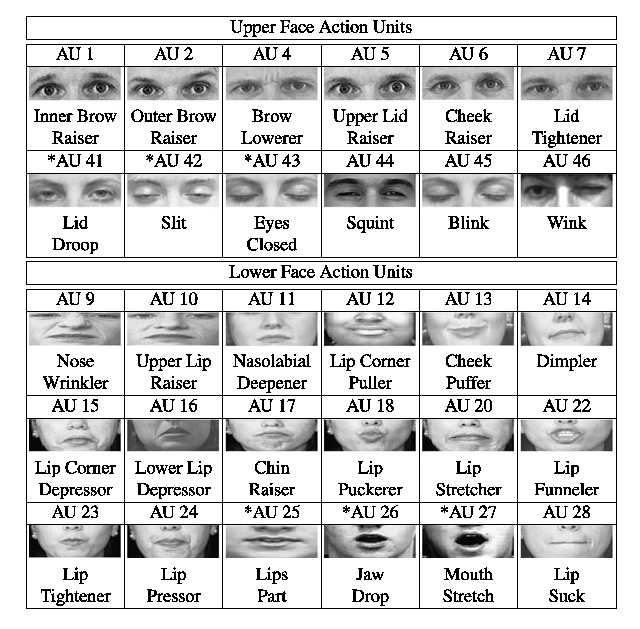
\includegraphics[scale=1]{./figures/faus.eps}
\caption{Facial Action Units}
\label{fig:fau}
\end{figure}

\subsubsection{Interpreting emotions}

\paragraph{Discrete case}
Emotions can roughly be broken down into six \textit{basic emotions} \cite{RefWorks:12}, seven if we count the neutral emotion. We can then interpret a facial expression into one of these seven categories. Note that this is only an interpretation as emotions are expressed though multiple channels such as body language or voice and facial expressions are only one of these channels.


\paragraph{Continuous case}
This is the case in which we are interested. Emotions can be represented using two continuous dimensions:

\begin{itemize}
\item \textbf{Valence}: characterises the attractiveness or aversivenes of an emotion, that is respectfully how positive or negative the emotion is.
\item \textbf{Arousal}: characterises the intensity of the emotion
\end{itemize}

We can therefore represent emotions in a two dimensional coordinate system using their valence and arousal values, see Figure ~\ref{fig:arval} 

\begin{figure}[h]
\centering
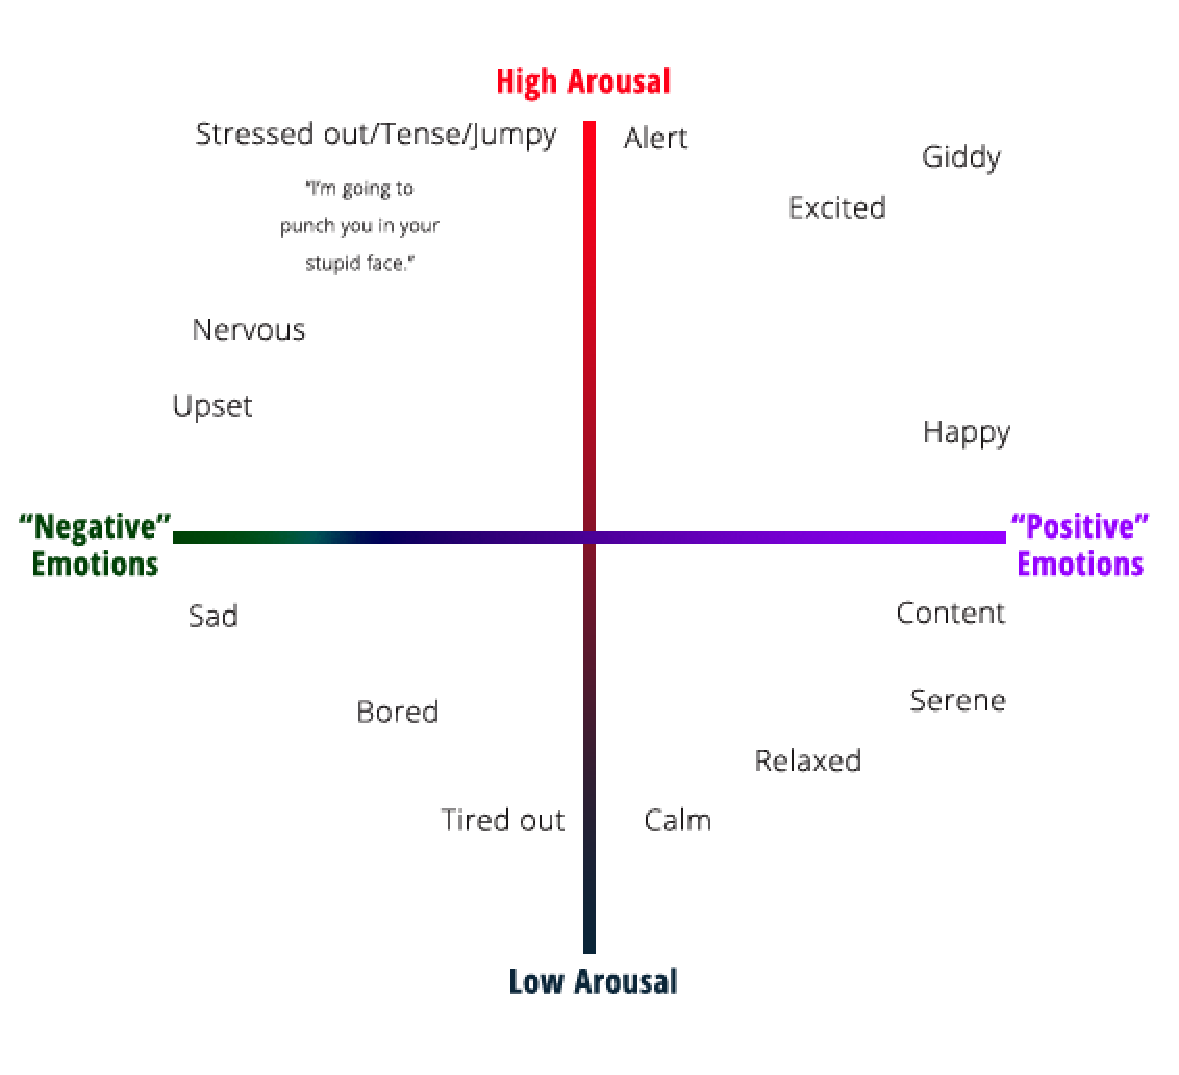
\includegraphics[scale=0.5]{./figures/valence_arousal_plot.eps}
\caption{Plotting emotions according to their valence and arousal}
\label{fig:arval}
\end{figure}

\begin{table}[h]
\centering
\begin{tabular}{|l|l|}
 \hline
 Emotion & AUs\\
 \hline
 Neutral   & 0                     \\
 Happiness & 6, 12                 \\
 Sadness   & 1, 4, 14              \\
 Surprise  & 1, 2, 5B, 26          \\
 Fear      & 1, 2, 4, 5, 7, 20, 26 \\
 Anger     & 4, 5, 7, 23           \\
 Disgust   & 9, 15, 16             \\
 \hline
\end{tabular}
\caption{The 6 basic emotions (plus neutral) and the corresponding Action Units that are generally activate when the emotion is present}
\label{tab:emo-au}
\end{table}

%%%%% EARLY DAYS %%%%%
\subsection{Facial Expression Analysis}

In the early days, facial expression analysis was restricted to recognising the six basic emotions. Furthermore, computer vision techniques were used to extract features from input images and then classify them instead of using the \textit{end-to-end} deep learning techniques we will use in this project. As indicated in \cite{RefWorks:2}, the interested reader is directed towards \cite{RefWorks:18,RefWorks:19} for a thorough overview of these early techniques.

\subsection{Databases}

We direct the reader towards \cite{RefWorks:2} for a complete survey of the main databases available for facial expression analysis. We are interested in databases containing images or videos taken in-the-wild and annotated with facial action units. A such, we will use the EmotioNet \cite{RefWorks:1} database which contains 1,000,000 in-the-wild images of emotions. These images were downloaded from the Internet by using specific combinations of keywords and were then automatically annotated with AUs and AU intensities as well as emotion categories by using a novel computer vision algorithm presented in \cite{RefWorks:1}. We also want to annotate valence and arousal, so we will be using the newly available Aff-Wild database \cite{RefWorks:2} which contains video taken in-the-wild (from YouTube) that have been manually annotated with valence and arousal.

For evaluation purposes, we will be using two databases:

\begin{itemize}
\item \textbf{DISFA} \cite{RefWorks:17}: videos of young adults watching video clips intended to elicit certain emotions. Although these videos are not in-the-wild since they were all recorded with the same stereo camera in similar lighting conditions, each frame has been manually annotated with AUs and their respective intensities.
\item \textbf{AMFED} \cite{RefWorks:18}: videos of people reacting to 3 chosen amusing Super Bowl commercials. The people were recorded using their laptop's web camera so the lighting conditions differ from one video to another. Furthermore, each frame was carefully annotated with a subset of facial action units.
\end{itemize}

\subsection{Deep Learning}

We use deep learning models in order to, given an image of a facial expression,
recognise which AUs are active and which aren't as well as estimate the valence and
arousal of the given facial expression. We use these models as they have proved
to be able to learn to represent abstract data features (e.g a smile) thanks to
multiple computational layers

\subsubsection{Deep Convolutional Neural Networks}

In particular, since our task focuses on images (i.e. 2/3-dimensional data), we
will be using a particular type of deep learning models called deep
convolutional neural networks (DCNNs). DCNNs consist of a succession of 
convolutional and pooling layers followed by fully connected layers.

The first block of layers, the convolutional and pooling layers, act as a feature
extractor. They take as input a raster image $\in \mathcal{R}^{nxm}$ where 
$n$ is the image height and $m$ the image width, either in greyscale ($\in
\mathcal{R}^{1xnxm}$) or in RGB colours $\in \mathcal{R}^{3xnxm}$ 
(where 3 is the depth of the image, i.e. the number of channels) and
processes it to extract features which will constitute a meaningful
representation of the image in a lower dimension, i.e. a vector.

\paragraph{Convolutional Layers}

Convolutional layers are the core components of DCNNs. They are were the most
heavy computations take place and act as feature extractors by applying a set
of spatially small learnable kernel filters to the input image. 
These filters could  for instance have a
size of 7x7x$D$ where the first and the second 7 correspond to the height and the
width of the filter respectively and $D$ corresponds to the depth (either 1 or 3
if we are working with RGB input images).

Each filter is applied by ``sliding'' it over the input image and performing a
convolution at every pixel of the image between the filter and the portion of 
the image that lies directly beneath it. Mathematically, this gives the
following: suppose we have an input image $I \in \mathcal{R}^{WxH}$ and a
filter $F \in \mathcal{R}^{kxk}$ such that $I(a,b)$ denotes the pixel on row
a and column b of $I$ (assume the same notation for $F$). Then the convolution
operation  $C(.,.)$ executed at pixel $(a,b)$ of the image is

\begin{equation}
  C(a,b) = \sum_{i=1}^{k}\sum_{j=1}^{k} F(i,j) \times I(a-i, b-j)
  \label{eq:convolution}
\end{equation}small

Therefore, as we slide a filter over the image, we produce a 2D response map
that corresponds to the convolved features at each spatial location of the
input image, see Fig.~\ref{fig:conv_op}. Intuitively, each kernel filter learns
to detect specific features in the input such as as corner or a blob of colour

In the case of a 3 dimensional input volume ($Width \times Height \times Depth$), each filter will also be 3
dimensional with the depth dimension $D$ matching that of the input. Therefore each
filter will produce $D$ response maps which are summed together with a bias
term to produce a 2 dimensional overall response map for that filter.

Finally, when using a $k\times k$ kernel on an $n \times m$ image, the response map will have a smaller
size of $(n-l)\times(m-l)$ where $l=\frac{k-1}{2}$ ($k$ is usually and odd
number). While we do want to perform dimensionality reduction before going
through the fully connected layers, this means that the kernel might omit some
important features that are at the edges of the image. To solve this problem,
it is common practice to add $l$ layers of zero-padding on each side of the
image so that the kernel also covers the edges of the image and the response
map has the same dimension as the input.

To sum up, here are the inputs and the outputs of a typical convolutional
layer with $N$ kernel features of size $k \times k$ applied using a stride of
$s$ on an image with a padding of $p$:

\begin{enumerate}
  \item \textbf{In}: an image with size $W \times H \times D$ where $W$ is the
    width of the image, $H$ the height and $D$ the depth
  \item \textbf{Out}: a volume with size $W_{out} \times H_{out} \times N$
    where $W_{out} = \frac{W - k + 2p}{s}$, $H_{out} = \frac{H- k + 2p}{s}$ and
    $N$ is the number of filters used at that layer
\end{enumerate}


\begin{figure}[ht]
  \centering
  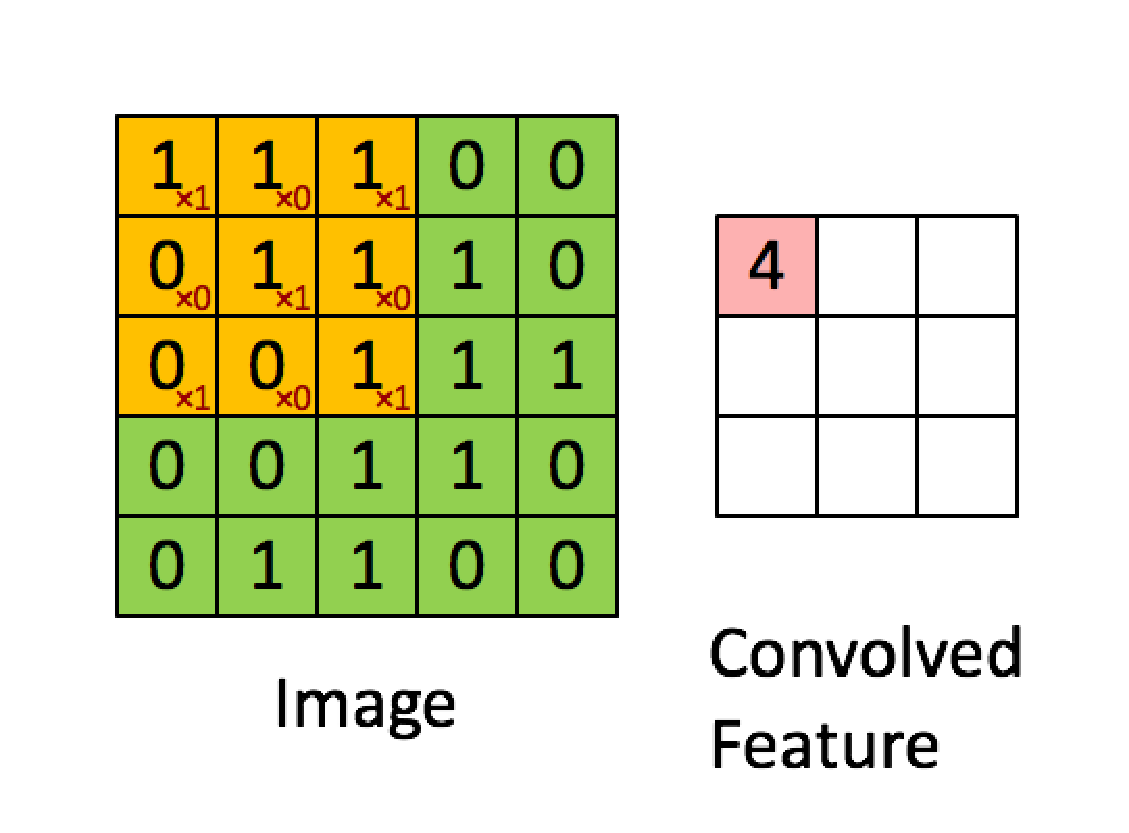
\includegraphics[scale=0.5]{./figures/convolution_example.eps}
  \caption{Example of a convolution operation at a single spatial location. The
  orange square represents the kernel filter. Note that no padding has been
applied here which is why the convolved feature (i.e. the response map) is
smaller.}
  \source{http://deeplearning.stanford.edu/wiki/images/6/6c/Convolution\_schematic.gif}
  \label{fig:conv_op}
\end{figure}

\paragraph{Pooling Layers}  

As mentioned in the above paragraph, convolutional layers can perform
dimensionality reduction if no zero-padding is added to the input image.
However this job generally falls to pooling layers.

As their name suggests, pooling layers group pixels together to reduce them to a
single pixel. There are several ways to determine the value of the output pixel
and the most common one is maximum pooling which consists in outputting the
pixel in the group that has the highest value. Since this is just a static
operation, there are no learnable parameters involved. The only parameters are
the spacial extent $p$ (i.e. the width and height) of the pooling region/filter and
the stride $s$ which defines how many pixels to skip until applying the next
pooling operation. For instance, a pooling layer with $p=2$ (2x2 filters) and
$s=2$ will divide the width and height of the input image by 2 (it does not
change the depth) as can be seen in Fig~\ref{fig:maxpool}.

\begin{figure}[ht]
  \centering
  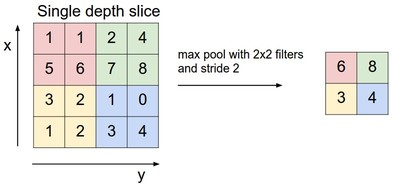
\includegraphics[scale=0.7]{./figures/maxpool.jpeg}
  \caption{example of a single max pooling operation with a $2 \times 2$ pooling
  filter and a stride of 2}
  \source{http://cs231n.github.io/assets/cnn/maxpool.jpeg}
  \label{fig:maxpool}
\end{figure}

To sum up here are the inputs and outputs of a pooling layer:

\begin{enumerate}
  \item \textbf{In}: $k$ images of size $n \times m \times d$ where $n$ is the
    width, $m$ the height and $d$ the depth of the image
  \item \textbf{Out}: $k$ responses of size $\left( \frac{n-p}{s} + 1  \right)\times
    \left( \frac{m-p}{s}+1  \right)\times d$ where $p$ is the width of the
    square pooling filter and $s$ the stride size
\end{enumerate}

\paragraph{Fully Connected Layers}

Fully connected layers constitute the second block of the 

Unlike convolutional layers, which are locally connected (each pixel in the
response map is locally connected to a sub-region of the input), fully
connected layers have their outputs connected to \textit{every} input.

As such, the activations can be simply calculated via matrix multiplication
between the inputs and their associated weights and adding a bias term before
passing all that to an activation function (e.g. ReLu, Sigmoid, Softmax).

It is worth noting that we can easily replace a fully connected layer by an
equivalent convolutional layer; all that must be done is to match the size of
the kernel filters to the size of the input image or vector. For instance, in
the VGG 16[CITE] network, the final convolutional layer outputs 512 feature maps of
size $7 \times 7$ which are passed on to a fully connected layer with 4096
neurons. Then we can replace this fully connected layer by a convolutional one
with 4096 filters of size $7 \times 7$

\paragraph{Dropout Layers}

Dropout layers[CITE] are a simple yet powerful regularisation technique to prevent,
overfitting. The key idea is to randomly block some neurons from connecting to
the next layer during training see Fig.~\ref{fig:dropout}. This prevents groups of neurons from
co-adapting too much and improves the flexibility of the network which
decreases overfitting.


\begin{figure}[ht]
  \centering
  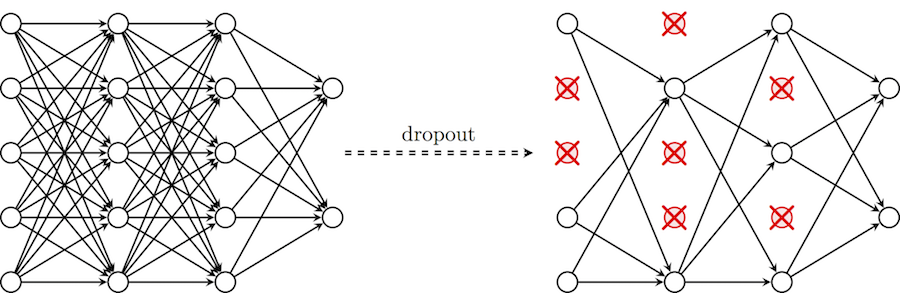
\includegraphics[scale=1]{./figures/dropout.png}
  \caption{example dropout layers: the crossed neurons are blocked from sending
  their inputs to the next layer}
  \source{https://cambridgespark.com/content/tutorials/convolutional-neural-networks-with-keras/figures/drop.png}
  \label{fig:dropout}
\end{figure}


\subsubsection{Optimisers}

\paragraph{Stochastic Gradient Descent}

\paragraph{SGD with Nesterov Momentum}

\paragraph{Adagrad}

\paragraph{RMSProp}

\paragraph{Adam}

\subsubsection{Activation functions}

\subsubsection{Models}

The reader is referred to \cite{RefWorks:2} (paragraph 3) for a review of existing deep learning methodologies for facial expression recognition "in-the-wild".

We  use two pre-existing and pre-trained models, namely \textbf{VGG} \cite{RefWorks:21} and
\textbf{ResNet} [CITE]. These were fine-tuned for specific tasks on our
database (a subset of the EmotioNet database[CITE])

\paragraph{VGG 16}

The VGG 16 network was developped by Karen Simonyan and Andrew Zisserman from
Oxford University's Visual Geometry Group and was the runner-up in ILSVRC 2014. 
The ``16'' signifies that there are 16 trainable (weight) layers: 13 convolutional
layers and 3 fully connected layers.

It's originality comes from the fact that it uses small kernel filters
($3 \times 3$) at each convolutional layer which are convolved with every
pixel of the input image (i.e. they use a stride of 1). Furthermore, 
the number of filters increases as we progress through the convolutional layers.
The idea behind this is to get the first layers to detect abstract features
such as lines and get the following layers to refine on that feature.

Finally all 5 max pool layers use a spacial exent of $p=2$ and a stride of
$s=2$ so that each pool layer divides the width and height of the input image
by 2 
 
\paragraph{Inception}

\section{EmotioNet Database}
 
\subsection{Downloading}

In order to use less space, the authors of the EmotioNet database do not offer
a direct download of the  around 25k images. Instead, they provide an xlsx file containing one line per image which consists of 61 columns: the first column corresponds to the URL of the image and the next 60 columns correspond to the 60 AUs in ascending order. To download the database, one must therefore read this file line by line, get the image at the specified URL and store it in a file. 

\subsubsection{Reading the xlsx file}

Python does not natively support the reading of xlsx files, and even though third party packages such as \textbf{openpyxl} by Eric Gazoni and Charlie Clark exist, we chose to convert the xlsx file containing the URLs and labels to a CSV file as these are easily readable in Python. One problem arose using this method, some URLs (less than 15) contained commas, meaning that the URL was split up into two or more columns which shifted the index of the AU values, thus giving an invalid label to the associated image. To remedy to this situation, we simply deleted all the commas from the URLs.

\subsubsection{Downloading the image}

Once we have retrieved the URL, we can get the raw image over the Internet by using the \textbf{urllib} library. This did not come without some complications as 2,760 images were not downloaded due to the errors listed below:

\begin{itemize}
\item HTTP 404 (Not Found) error: 1,726 URLs
\item HTTP 400, 401, 403, 410 errors: 205 URLs
\item HTTP 500, 502, 503, 504 errors: 102 URLs
\item HTTP 301, 302 errors: 20 URLs
\item Name or service not known: 500 URLs
\item Connection timed out: 109 URLs
\item Connection reset by peer: 17 URLs
\item Connection refused: 16 URLs
\item No route to host: 10 URLs
\item Certificate verify failed: 14 URLs
\end{itemize}

The \textit{Name or service not known} errors can be caused by the lack of an internet connection which can occur when downloading via Wi-Fi. Because of this, some valid URLs will not be accessed to download an image. To solve this problem, we keep track of which images remain to be downloaded by taking all the URLs and removing those that were already downloaded as well as those that led to an error and launch the download script again. To keep track of the erroneous URLs, each time an URL leads to an error, it is stored along with its error in a text file and to construct the list of already downloaded images, we just list the files present in the specified download directory.

\subsubsection{Storing the image}

Storing the fetched raw image implies creating a file and more importantly naming it in such a way that using this name, we can retrieve the associated label (AU values) from the xlsx file. We initially used an URL parser to extract the query component of the URL which should consist of the name of the image (e.g. image.jpeg). However, it turns out that this query component can also have a parameter component (e.g "?size=200x200" in HTTP://www.foo.com/bar/image.jpeg?size=200x200). So converting the URL into a file name based solely on the query component of the URL meant that two different URLs/images could lead to the exact same file name when we require this \texttt{url\_to\_filename} function to be a bijection in order to be able to retrieve the associated label from the xlsx file.

We therefore abandoned this method and just used the URL with a couple of preprocessing steps as file name. The preprocessing steps consisted in removing full stops from the URL and replacing forward slashes with underscores as they would otherwise be understood as directories by the file system. Additionally, we determine the type of the ray image (e.g. png, jpeg, gif ...) and append it to the file name. Finally, file names cannot be longer than 250 chars on most systems so we truncate the beginning of URLs that violate this limit.

\subsection{Converting to TFRecords}

TFRecords is the standard recommended file format to store data that will be used by a TensorFlow network or Graph. It is based on Google's Protocol Buffers which are language and platform agnostic object serialisation mechanisms. 

Converting a data set to a set of TFRecord files is no easy task, but thankfully TensorFlow provides a script, \texttt{build\_image\_data.py}, that does just that and only needed a few modifications to adapt it to the nature of our data set. Indeed, this script provided by TensorFlow was used to convert the images of the CIFAR-10[CITE] database and relied on a special organisation of the data to assign labels: one eponymous subdirectory should be created for each image category (label) and all the images of that category should be placed into that subdirectory (e.g. and image of a cat would be in the /dataset/cat/ subdirectory). However this mechanism does not apply in our case since it assumes that the categories are mutually exclusive (one image cannot be categorised as a cat and a dog at the same time) to partition the data set into subdirectories, whereas in our case, an image can have multiple active AUs at once.

So we had to change the way the script assigned labels to images by constructing a dictionary of URLs to labels using the xlsx data file and then using the file name of the image to look up its label in this dictionary. We also had to change the way the label was stored in the TFRecord as it now consist of an array of \texttt{int64} rather than a single \texttt{int64}. Finally, the script converts andy PNG image to JPEG for consistency, however, it does not handle other image types such as GIF so we added the necessary logic to convert GIFs to JPEG images.

The script then takes care of multi-threading for efficiency and outputs a training and a validation TFRecord file, both split into a number of user-specified shards.

\subsection{Extending TF-Slim datasets}

Having downloaded the datbase and converted it to TFRecord format, we now
extend the TF-Slim datasets to incorporate ours. This has many advantages as
TF-Slim then takes care of creating a data provider for our models and more
importantly, it allows us to easily reuse TF-Slim's generic training and
evaluation scripts.

In order to do this, we created a new file in \texttt{/slim/datasets/} called \texttt{images.py} 
which returns an instance of a TF-Slim Dataset class, customised for our dataset. 
We then add this instance to the \texttt{dataset\_factory} file's dictionnary.
Our dataset can now be accessed using the
\texttt{dataset\_factory.get\_dataset()} method which only requires the name of
the dataset, the path to the actual data and the name of the split to use (one
of 'train' or 'validation'). This means that we can easily change data sets,
should we add some in the future and makes our training and evaluating system
more modular.

\subsection{Annotating Valence and Arousal}

As mentioned in section [CITE], this database was annotated by human annoators
on Action Unit presence/absence only. However, we are also intereseted in
valence and arousal values as it is believed that the presence or absence of
AUs is correlated to the valence and arousal of the emotion that can be
interpreted from a facial expression.

As such, one of the major tasks, was to first annotate the 21,500 images that
were downloaded with both valence and arousal. This was done using a tool
available for research purpose only and developed by J. Kossaifi, 
G. Tzimiropoulos, S. Todorovic and M. Pantic. This tool was designed to
annotate videos, not large image data sets, so we first divided the 21,500
images into 21 videos of 1000 frames and a 22nd video of 500 frames. You then
load up a video and start annotating the frames for valence. Once all the
frames of the video are annotated with valence, we annotate them with arousal
and move on to the next video.

\section{Action Unit Classification}

This task was performed on the full data set

\subsection{VGG 16}

\subsection{ResNet}

\section{Valence and Arousal Regression}

\subsection{VGG 16}

\subsection{ResNet}








% REFERENCES
\clearpage
\bibliographystyle{plain}
\bibliography{refs.bib}

\appendix


\end{document}
%%% Local Variables: 
%%% mode: latex
%%% TeX-master: t
%%% End: 
